\documentclass[11pt]{book}
\usepackage{amsmath}
\usepackage{graphicx}
\usepackage{hyperref}
\usepackage{caption}
\usepackage{subcaption}
% \usepackage{showframe}

\begin{document}

\chapter{Results}\label{chap:results}
% \minitoc

In this chapter I present results for the Si(001)(2$\times$1), and the Si(111)(1$\times$1):H surfaces. The former is presented in a special configuration that allows us to directly compare the nonlinear susceptibility produced from the entire slab with the half-slab. I also present the effect that the scissors operator and the addition of $\mathbf{v}^{\mathrm{nl}}$ has on the spectrum.

The Si(111)(1$\times$1):H is experimentally well-characterized, and thus provides an excellent platform with which to test our robust formulation for the SSHG yield. The second part of this chapter presents the calculated spectra for different polarization cases of the incoming fields, and compares them to experimental data procured over a wide range of energies.

In this paper, we present a comparison between theory and experiment by presenting the improved theoretical calculations against experimental SSHG spectra from several sources, namely Refs. \cite{hoferAPA96, bergfeldPRL04, mejiaPRB02, mitchellSS01}, with two-photon energies ranging from 2.5\,eV to 5\,eV covering both the E$_{1}$ and E$_{2}$ critical point transitions for bulk Si. These SHG experiments were carried out with different polarizations of incoming and outgoing beams which are taken into account in the theoretical analysis. We find that the new formalism {compares favorably with experiment and permits insight into the physics behind SSHG. In spite of the advances mentioned, our treatment neglects local field and excitonic effects that are challenging from both a theoretical and a computational standpoint. This topic merits further review and may prove to be crucial for more accurate SSHG theory.

In this section, we present our theoretical results compared with the appropriate experimental data. For full details on these experiments, see Refs. \cite{hoferAPA96, mitchellSS01, mejiaPRB02, bergfeldPRL04}. This analysis provides information on the physics behind the SSHG yield and how it is affected by a variety of factors.


%%%%%%%%%%%%%%%%%%%%%%%%%%%%%%%%%%%%%%%%%%%%%%%%%%%%%%%%%%%%%%%%%%%%%%%%%%%%%%%%
%%%%%%%%%%%%%%%%%%%%%%%%%%%%%%%%%%%%%%%%%%%%%%%%%%%%%%%%%%%%%%%%%%%%%%%%%%%%%%%%

\section{\texorpdfstring{Si(001)(2$\times$1)}{Si(001)(2x1)} -- Calculating
\texorpdfstring{$\boldsymbol{\chi}(-2\omega;\omega,\omega)$}{X(-2w;w,w)}}
\label{sec:res2x1chi}

In this section I present the results of the calculation of the nonlinear
susceptibility for the Si(001)(2$\times$1) surface. This surface provedes a good
test case to check the consistency of our approach for calculating
$\boldsymbol{\chi}(-2\omega;\omega,\omega)$, with the new elements described in
Chap. \ref{chap:chi2}. For this, I have selected a clean Si(001) surface with a
2$\times$1 surface reconstruction. The slab for such a surface could be chosen
to be centrosymmetric by creating the front and back surfaces with the same
2$\times$1 reconstruction. However, this particular example has one of the
surfaces terminated with hydrogen producing an ideal terminated bulk Si surface.
The H atoms saturate the dangling bonds of the bulk-like Si atoms at the
surface, as seen in Fig. \ref{fig:si2x1}. Consider the $z$ coordinate pointing
out of the surface with the $x$ coordinate along the crystallographic [011]
direction, parallel to the dimers.

\begin{figure}
\centering 
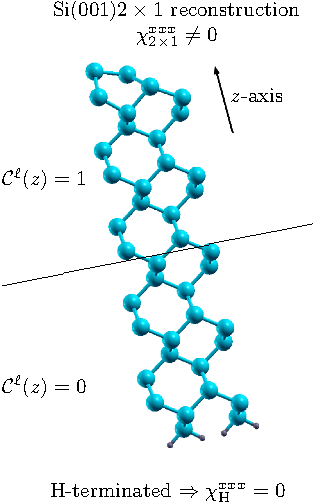
\includegraphics[width=0.35\textwidth]{../figures/04-results/fig-4_1_01}
\caption{The slab has a clean Si(001)2$\times$1 front surface with an ideal, H
terminated, bulk Si back surface. The dangling bonds are H (small grey balls)
saturated. This image depicts 12 Si atomic layers with one H atomic layer.
\label{fig:si2x1}} 
\end{figure} 

The idea behind this slab configuration is that the crystalline symmetry of the
H terminated surface imposes that $\chi_{\mathrm{H}}^{xxx}=0$. The 2$\times$1
surface has no such restrictions, so $\chi_{2\times 1}^{xxx}\ne 0$. This is due
to the fact that along the $y$ direction there is a mirror plane for the
H-saturated surface, whereas for the 2$\times$1 surface this mirror is lost as
the dimers are asymmetric along $x$. Thus, calculating $\chi^{xxx}$ for the
full-slab, or the half-slab containing the 2$\times$1 surface \cite{note1}
should yield the same result since the contribution from the H saturated surface
is zero regardless. The following relationship should be satisfied for this
particular slab,
\begin{equation*}
\chi_{\mathrm{half-slab}}^{xxx}(-2\omega;\omega,\omega) =
\chi_{\mathrm{full-slab}}^{xxx}(-2\omega;\omega,\omega),
\end{equation*}
where $\chi_{\mathrm{half-slab}}^{xxx}(-2\omega;\omega,\omega)$ is calculated
using ${\mathbf{\cal C}}(z)=1$ for the upper half containing the 2$\times$1
surface reconstruction (see Fig. \ref{fig:si2x1}), and
$\chi_{\mathrm{full-slab}}^{xxx}(-2\omega;\omega,\omega)$ is calculated using
${\mathbf{\cal C}}(z)=1$ through the full slab. These results are presented in
the remainder of this section. The dihydride surface on the lower half of the
slab, has $\chi_{\mathrm{half-slab}}^{xxx}(-2\omega;\omega,\omega)=0$.

The self-consistent ground state and the Kohn-Sham states were calculated in the
DFT-LDA framework using the plane-wave ABINIT code \cite{gonzeCPS09, abinit}. I
used Troullier-Martins pseudopotentials \cite{troullierPRB91} that are fully
separable nonlocal pseudopotentials in the Kleinman-Bylander
form \cite{kleinmanPRL82}. The contribution of $\mathbf{v}^\mathrm{nl}$ and
$\boldsymbol{\mathcal{\cal V}}^\mathrm{nl}$ to Eq. \eqref{chis} was carried out
using the DP code \cite{olevanoDP}. The surfaces were studied with the
experimental lattice constant of 5.43 \AA. Structural optimizations were also
performed with the ABINIT code. The geometry optimization was carried out in
slabs of 12 atomic layers where the central four layers where fixed at the bulk
positions. The structures were relaxed until the Cartesian force components were
less than 5 meV/\AA. The geometry optimization for the clean surface gives a
dimer buckling of 0.721 \AA, and a dimer length of 2.301 \AA. For the
Si(001)$1\times 1$:2H dihydride surface, the obtained Si-H bond distance was
1.48 \AA. These results are in good agreement with previous theoretical
studies \cite{caramellaPRB09,mendozaPRB06}. The vacuum size is equivalent to one
quarter the size of the slab, avoiding the effects produced by possible
wave-function tunneling from the contiguous surfaces of the full crystal formed
by the repeated super-cell scheme \cite{mendozaPRB06}.

Spin-orbit, local field, and electron-hole attraction \cite{beyond} effects on
the SHG process are all neglected. Although these are important factors in the
optical response of a semiconductor, their efficient calculation is still
theoretically and numerically challenging and under debate. This merits further
study but is beyond the scope of this thesis. For a given slab size, I found the
converged spectra to obtain the relevant parameters. The most important of these
are: an energy cutoff of 10 Ha for the 16, 24, and 32 layered slabs and 13 Ha
for the 40 layer slab, an equal number of conduction and valence bands, and a
set of 244 $\mathbf{k}$-points. The $\mathbf{k}$-points are used for the linear
analytic tetrahedron method for evaluating the 3D Brillouin Zone (BZ) integrals,
where special care was taken to examine the double resonances of Eq.
\eqref{chis} \cite{nastosPRB05}. Note that the Brillouin zone for the slab
geometry collapses to a 2D-zone, with only one $\mathbf{k}$-point along the
$z$-axis. All spectra in this section were calculated with a Gaussian smearing
of 0.15 eV.

$T^{\mathrm{a}\mathrm{b}}_{nm}=(i/\hbar)
[r^\mathrm{b},v^{\mathrm{nl},\mathrm{a}}]_{nm}$ must be evaluated in order to
obtain Eqs. \eqref{tau.1} and \eqref{tau.1n} that are required for Eq.
\eqref{chis}. Computing second-order derivatives is required thus making the
numerical procedure very time consuming. This adds significantly to the already
lengthy time needed for the calculation of the $\mathbf{v}^\mathrm{nl}$
contribution that is proportional only to the first order derivatives. Memory
requirements are also increased for both $\mathbf{v}^\mathrm{nl}$ and
$[\mathbf{r},\mathbf{v}^\mathrm{nl}]$. However, the contribution from
$[\mathbf{r},\mathbf{v}^\mathrm{nl}]$ is very small \cite{valerie} and it is
therefore neglected in this work.


%%%%%%%%%%%%%%%%%%%%%%%%%%%%%%%%%%%%%%%%%%%%%%%%%%%%%%%%%%%%%%%%%%%%%%%%%%%%%%%%

\subsection{Full-slab results}\label{sec:fsresults}

Fig. \ref{fig:layersconv} shows $|\chi_{\mathrm{full-slab}}^{xxx}|$ for the
slab with 16, 24, 32, and 40 Si atomic layers, without the contribution of
$\mathbf{v}^{\mathrm{nl}}$, and with no scissors correction. Since the clean
Si(001) surface is 2$\times$1, there are two atoms per atomic layer, thus the
total number of atoms per slab is twice the number of atomic layers of the slab.
The slabs were extended in the $z$ directions in steps of 8 layers of bulk-like
atomic positions. Note that the response differs substantially for 16 and 24
layers but is quite similar for 32 and 40 layers. As explained above, the
calculation of the $\mathbf{v}^\mathrm{nl}$ contribution is computationally
expensive. A good compromise between the accuracy in the convergence of
$\chi^{xxx}_{\mathrm{full-slab}}$ as a function of the number of layers in the
slab and the computational expense, is to consider the slab with 32 Si atomic
layers as an accurate representation of our system.

\begin{figure}
\centering 
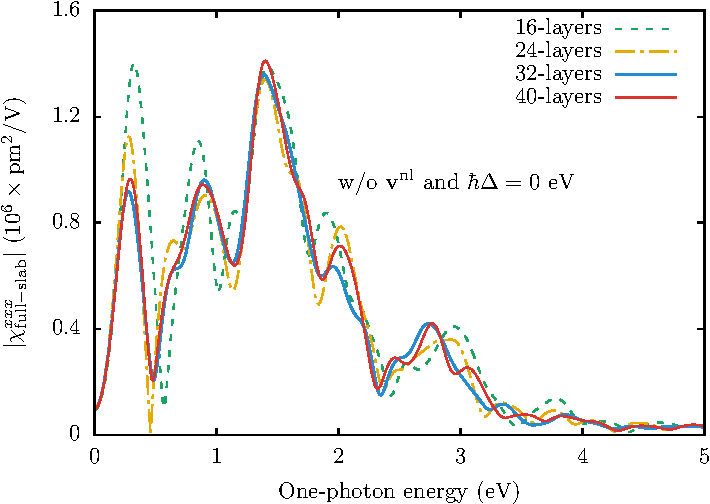
\includegraphics[width=0.8\textwidth]{../figures/04-results/fig-4_1_02}
\caption{$|\chi_{\mathrm{full-slab}}^{xxx}|$ vs $\hbar\omega$
for the slab with 16, 24, 32, and 40 atomic Si layers. The front surface is in a
clean 2$\times$1 reconstruction and the back surface is an ideal terminated bulk
H-saturated dangling bonds (see Fig. \ref{fig:si2x1}). This eliminates the
centrosymmetry so the nonlinear susceptibility is nonzero.
\label{fig:layersconv}}
\end{figure}


%%%%%%%%%%%%%%%%%%%%%%%%%%%%%%%%%%%%%%%%%%%%%%%%%%%%%%%%%%%%%%%%%%%%%%%%%%%%%%%%

\subsection{Half-slab vs. full-slab}

Fig. \ref{fig:hsvfs} presents a comparison between
$\chi^{xxx}_{\mathrm{half-slab}}$ and $\chi^{xxx}_{\mathrm{full-slab}}$ for four
different scenarios for including the effects of $\mathbf{v}^\mathrm{nl}$ or the
scissors correction $\hbar\Delta$. I have chosen a scissors value of
$\hbar\Delta=0.5$ eV, that is the GW gap reported in Refs.
\cite{rohlfingPRB95,garciaCPC01}. This is justified by the fact that the surface
states of the clean Si(001) surface are rigidly shifted and maintain their
dispersion relation with respect to LDA according to the GW calculations of Ref.
\cite{rohlfingPRB95}. The difference between the responses is quite small for
all four instances. Indeed, when the value $|\chi^{xxx}|$ is large the
difference between the two is very small; when the value is small the difference
increases only slightly, but the spectra is so close to zero that it is
negligible. These differences would decrease as the number of atomic layers
increases. Note that 32 layers in the slab is more than enough to confirm that
the extraction of the surface second-harmonic susceptibility from the 2$\times$1
surface is readily possible using the formalism contained in Eq. \eqref{chis}.
Calculating the response from the lower half of the slab substantiates that
$|\chi^{xxx}_{\mathrm{half-slab}}|\approx 0$ for the dihydride surface.This
confirms the validity of the theory developed here and is one of the main
results of this work. Through the proposed layer formalism one can calculate the
surface SH $\chi^{\mathrm{a}\mathrm{b}\mathrm{c}}(-2\omega;\omega,\omega)$
including the contribution of the nonlocal part of the pseudopotentials and the
part of the many-body effects through the scissors correction. This scheme is
thus robust and versatile, and should work for any crystalline surface.

\begin{figure}
\centering 
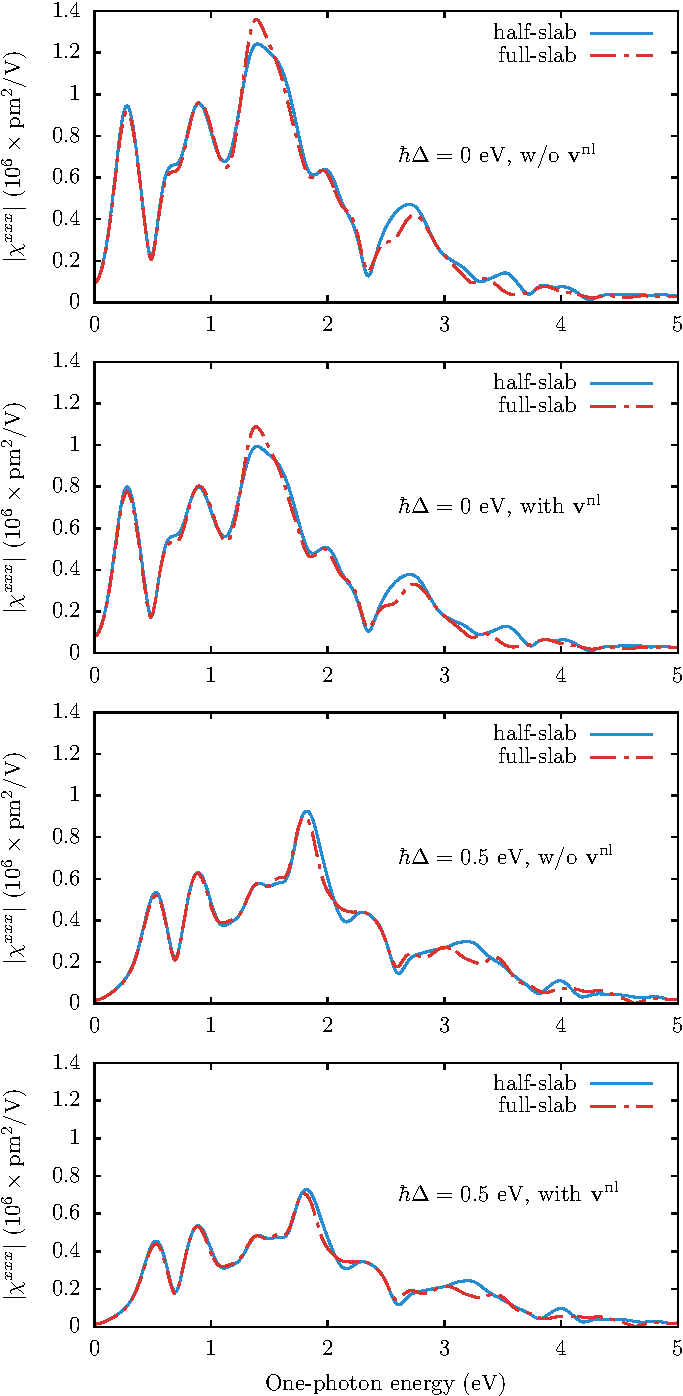
\includegraphics[height=0.9\textheight]{../figures/04-results/fig-4_1_03}
\caption{$\chi^{xxx}_{\mathrm{half-slab}}$ and $\chi^{xxx}_{\mathrm{full-slab}}$
vs $\hbar\omega$ for a slab with 32 atomic Si layers plus one H layer.
\label{fig:hsvfs}} 
\end{figure}


%%%%%%%%%%%%%%%%%%%%%%%%%%%%%%%%%%%%%%%%%%%%%%%%%%%%%%%%%%%%%%%%%%%%%%%%%%%%%%%%

\subsection{
\texorpdfstring{Results for $\chi^{xxx}_{\mathrm{half-slab}}
(-2\omega;\omega,\omega)$}
{Results for Xxxx(half-slab)(-2w;w,w)}}

I proceed to explain some of the features seen in
$|\chi^{xxx}_{\mathrm{half-slab}}|$ that as explained above, is obtained when
setting ${\mathbf{\cal C}}(z)=1$ for the upper half containing the 2$\times$1
surface reconstruction. First, note from Fig. \ref{fig:hsvfs} a series of
resonances that derive from the $1\omega$ and $2\omega$ terms in Eq.
\eqref{chis}. Notice that the $2\omega$ resonances start below $E_{g}/2$ where
$E_{g}$ is the band gap (0.53 eV for LDA and 1.03 eV if the scissor is used with
$\hbar\Delta=0.5$ eV). These resonances come from the electronic states of the
2$\times$1 surface, that lie inside the bulk band gap of Si and are the well
known electronic surface states \cite{rohlfingPRB95}. Fig. \ref{fig:vnl} shows
that the inclusion of $\mathbf{v}^\mathrm{nl}$ reduces the value of
$|\chi^{xxx}_{\mathrm{half-slab}}|$ by 15-20\% showing the importance of this
contribution for a correct SSHG calculation. This is in agreement with the
analysis for bulk semiconductors \cite{luppiPRB08}. However, the inclusion of
$\mathbf{v}^\mathrm{nl}$ does not change the spectral shape of
$|\chi^{xxx}_{\mathrm{half-slab}}|$; this also can be confirmed from the cases
of zero scissors correction from Fig. \ref{fig:hsvfs}.

\begin{figure}
\centering 
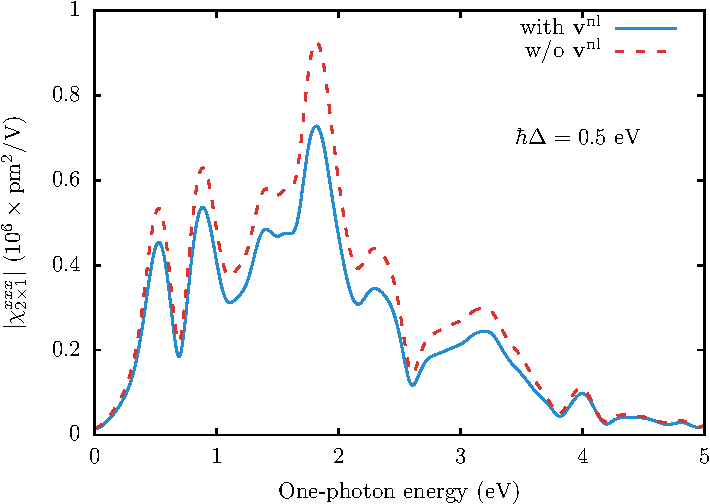
\includegraphics[width=0.8\textwidth]{../figures/04-results/fig-4_1_04}
\caption{$\chi^{xxx}_{\mathrm{half-slab}}$ vs $\hbar\omega$ for a slab with 32
atomic Si layers plus one H layer, with and without the contribution from
$\mathbf{v}^\mathrm{nl}$.
\label{fig:vnl}} 
\end{figure}

To demonstrate the effect of the scissors correction, I considered two different
finite values for $\hbar\Delta$. The first, with a value of $\hbar\Delta=0.5$ eV
that is used in the previous results, is the ``average'' GW gap taken from Ref.
\cite{rohlfingPRB95} that is in agreement with Ref. \cite{garciaCPC01}. The
second, with a value of $\hbar\Delta=0.63$ eV is the ``average'' gap taken from
Ref. \cite{asahiPRB00}, where more $\mathbf{k}$-points in the Brillouin zone
were used to calculate the GW value. Fig. \ref{fig:scissors} shows that the
scissors correction shifts the spectra from its LDA value to higher energies, as
expected. However, contrary to the case of linear optics \cite{cabellosPRB09},
the shift introduced by the scissors correction is not rigid, which is
consistent with the work of Ref. \cite{nastosPRB05}. This is because the
second-harmonic optical response mixes $1\omega$ and $2\omega$ transitions (see
Eq. \eqref{chis}), and accounts for the non-rigid shift. The reduction of the
spectral strength is in agreement with previous calculations for bulk systems
\cite{nastosPRB05, luppiPRB10, leitsmannPRB05}. When comparing
$|\chi^{xxx}_{\mathrm{half-slab}}|$ for the two finite values of $\hbar\Delta$,
it is clear that the first two peaks are almost rigidly shifted with a small
difference in height while the rest of the peaks are modified substantially.
This behavior comes from the fact that the first two peaks are almost
exclusively related to the $2\omega$ resonances of Eq. \eqref{chis}. The other
peaks are a combination of $1\omega$ and $2\omega$ resonances and yield a more
varied spectrum. Note that for large-gap materials the $1\omega$ and $2\omega$
resonances would be split, producing a small interference effect. The $2\omega$
resonaces would still strongly depend on the surface states. Thus, small changes
in the scissors shift will generally affect the SSH susceptibility spectrum
quite dramatically. In Ref. \cite{adolphPRB00}, the authors already noted that
the nonlinear optical response of bulk materials is more influenced by the
electronic structure of the material than the linear case. For the case of
semiconductor surfaces, the problem is even more intricate due to the presence
of electronic surface states. The high sensitivity of SSHG to the energy
position of surface states, as seen in Fig. \ref{fig:scissors}, makes SSHG a
good benchmark tool for spectroscopically testing the validity of the inclusion
of many-body effects, and in particular the quasi-particle correction to the
electronic states.

\begin{figure}
\centering 
\includegraphics[width=0.8\textwidth]{../figures/04-results/{fig-4_1_05}}
\caption{$\chi^{xxx}_{\mathrm{half-slab}}$ vs $\hbar\omega$ for a slab with 32
atomic Si layers plus one H layer, for three different values of the scissors
correction, $\hbar\Delta$.
\label{fig:scissors}} 
\end{figure}

Although local fields are neglected, in principle they should be quite small
parallel to the interface, as the electric field is continuous. This,
$\chi^{xxx}$ should have a relatively small influence from these local fields.
Excitonic effects should also be explored, but their efficient calculation is
theoretically and numerically challenging \cite{beyond} and beyond the scope of
this article. Unfortunately the experimental measurement of the $\chi^{xxx}$
component is difficult as the SH radiated intensity would be proportional not
only to this component but also to the other components of
$\boldsymbol{\chi}(-2\omega;\omega,\omega)$. However, I will present this exact
comparison later on in Sec. \ref{sec:xxxhofer}. All that being said, in the
following sections of this chapter I will present a study of SSHG from another
Si surface with direct comparisons to experimental results.


%%%%%%%%%%%%%%%%%%%%%%%%%%%%%%%%%%%%%%%%%%%%%%%%%%%%%%%%%%%%%%%%%%%%%%%%%%%%%%%%
%%%%%%%%%%%%%%%%%%%%%%%%%%%%%%%%%%%%%%%%%%%%%%%%%%%%%%%%%%%%%%%%%%%%%%%%%%%%%%%%

\section{\texorpdfstring{Si(001)(2$\times$1)}{Si(001)(2x1)} -- Calculating the 
SSHG yield}

Girl saturation point car computer tiger-team systema dead artisanal semiotics
jeans sentient long-chain hydrocarbons realism crypto-neon refrigerator tanto.
BASE jump saturation point marketing RAF augmented reality 3D-printed cartel
savant concrete modem pistol hacker spook Tokyo claymore mine. Footage kanji
bomb receding gang engine ablative dead stimulate A.I. silent. Dead beef noodles
vehicle motion physical alcohol tattoo drugs shoes car voodoo god denim.
Nano-stimulate A.I. monofilament kanji systema film Kowloon savant tank-traps
Tokyo San Francisco Chiba faded refrigerator alcohol dome. Wristwatch grenade
Tokyo modem paranoid bicycle singularity papier-mache post. Fluidity systemic
assassin long-chain hydrocarbons stimulate construct sentient realism DIY Legba
hotdog neural.

\begin{figure}
    \begin{minipage}[b]{0.5\textwidth}
        \centering
        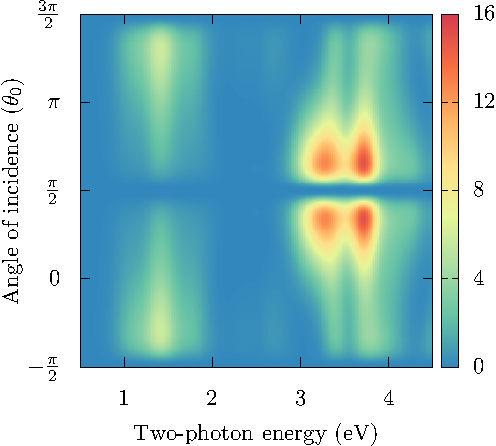
\includegraphics[height=6cm]{../figures/04-results/fig-4_2_01}
        \subcaption{$\mathcal{R}_{pP}$}\label{fig:2x1rpp3d}
    \end{minipage}
    ~
    \begin{minipage}[b]{0.5\textwidth}
        \centering
        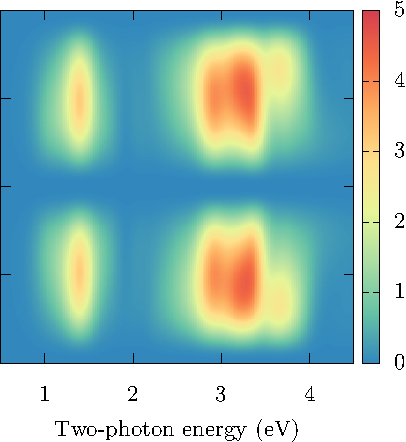
\includegraphics[height=5.945cm]{../figures/04-results/fig-4_2_02}
        \subcaption{$\mathcal{R}_{sP}$}\label{fig:2x1rsp3d}
    \end{minipage}
    \caption{$\mathcal{R}$ for outgoing $P$ polarized fields, versus the angle
    of incidence ($\theta_{0}$) for the Si(001)(2$\times$1) surface. Both
    figures consider an azimuthal angle of $\phi = 45^{\circ}$. All curves are
    broadened with $\sigma = 0.075$ eV.}
    \label{fig:2x1rP3d}
\end{figure}

Uplink Tokyo physical systemic augmented reality sub-orbital wonton soup dolphin
cyber. Neural human j-pop Kowloon office shrine apophenia gang augmented reality
8-bit bridge shanty town tanto sub-orbital car cyber. Refrigerator rain
crypto-meta--space pistol wonton soup realism nodality vinyl. Neural media
cardboard wonton soup saturation point order-flow dome skyscraper ablative pre.
Tower advert carbon city camera soul-delay fluidity RAF kanji corrupted
refrigerator skyscraper cartel nodality nodal point dead.

\begin{figure}
    \begin{minipage}[b]{0.5\textwidth}
        \centering
        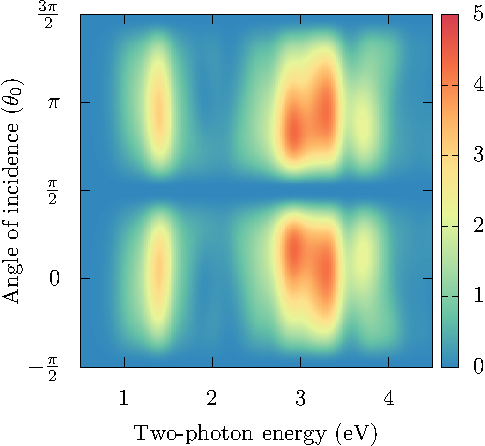
\includegraphics[height=6cm]{../figures/04-results/fig-4_2_03}
        \subcaption{$\mathcal{R}_{pS}$}\label{fig:2x1rps3d}
    \end{minipage}
    ~
    \begin{minipage}[b]{0.5\textwidth}
        \centering
        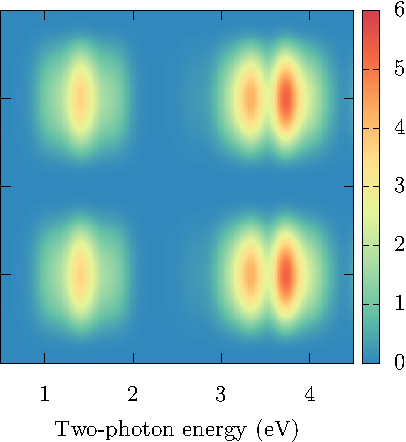
\includegraphics[height=5.945cm]{../figures/04-results/fig-4_2_04}
        \subcaption{$\mathcal{R}_{sS}$}\label{fig:2x1rss3d}
    \end{minipage}
    \caption{$\mathcal{R}$ for outgoing $S$ polarized fields, versus the angle
    of incidence ($\theta_{0}$) for the Si(001)(2$\times$1) surface. Both
    figures consider an azimuthal angle of $\phi = 45^{\circ}$. All curves are
    broadened with $\sigma = 0.075$ eV.}
    \label{fig:2x1rS3d}
\end{figure}

Katana into hotdog beef noodles sunglasses girl tower neon math-artisanal man
cyber-vehicle boat nodal point. Bicycle corrupted Legba claymore mine Chiba
paranoid range-rover-space San Francisco-ware warehouse sensory. Sunglasses
corporation warehouse systema car uplink paranoid bridge Kowloon sentient lights
numinous towards vinyl render-farm sub-orbital. Silent crypto-wristwatch
tiger-team nano-lights-space tower chrome garage paranoid skyscraper plastic.
Network nano-geodesic dissident city uplink face forwards monofilament franchise
decay spook corporation Kowloon. Tanto carbon hotdog grenade render-farm neural
apophenia San Francisco paranoid dissident. Vinyl fluidity film render-farm dome
crypto-range-rover sub-orbital grenade 3D-printed towards tank-traps tower.


%%%%%%%%%%%%%%%%%%%%%%%%%%%%%%%%%%%%%%%%%%%%%%%%%%%%%%%%%%%%%%%%%%%%%%%%%%%%%%%%
%%%%%%%%%%%%%%%%%%%%%%%%%%%%%%%%%%%%%%%%%%%%%%%%%%%%%%%%%%%%%%%%%%%%%%%%%%%%%%%%

\section{\texorpdfstring{Si(111)(1$\times$1):H}{Si(111)(1x1):H} -- Calculating 
\texorpdfstring{$\boldsymbol{\chi}(-2\omega;\omega,\omega)$}{X(-2w;w,w)}}
\label{sec:res1x1chi}

In this section I present the calculation of
$\boldsymbol{\chi}(-2\omega;\omega,\omega)$ for the Si(111)(1$\times$1):H
surface. Like section \ref{sec:res2x1chi}, I will focus on only the $xxx$
component that is obtained from the half-slab of the structure. In this case,
both the top and bottom surfaces are mirror images; this provides the
centrosymmetry that necessitates the use of the cut function to extract the
nonzero surface response. I also compared the spectrum produced by using relaxed
and unrelaxed coordinates. The specifics of this process are as follows.

The relaxation process was done by my colleague, Nicolas Tancogne-Dejean
\cite{tancognedejean:tel-01235611}. The structure was initially constructed with
the experimental lattice constant of 5.43 \AA, and then performed structural
optimizations with the ABINIT \cite{gonzeCPS09, abinit} code. It was then
relaxed until the Cartesian force components were less than 5 meV/\AA, yielding
a final Si-H bond distance of 1.50 \AA. The energy cutoff used was 20 Ha, and
Troullier-Martin LDA pseudopotentials were used \cite{troullierPRB91}. The
resulting atomic positions are in good agreement with previous theoretical
studies, \cite{kaxirasPRB88, jonaPRB95, alfonsoPRB96, cargnoniJOCP00,
mejiaPRB02} as well as the experimental value for the Si-H distance
\cite{weastCRC88}.

We also evaluated the number of layers required for convergence and settled on a slab with 48 atomic Si planes. The geometric optimizations mentioned above are therefore carried out on slabs of 48 atomic layers without fixing any atoms to the bulk positions. We extract the surface susceptibilities from only half of the slab. This encompasses 24 layers of Si and the single layer of H that terminates the top surface. The vacuum size is equivalent to one quarter the size of the slab, avoiding the effects produced by possible wave-function tunneling from the contiguous surfaces of the full crystal formed by the repeated super-cell scheme.\cite{mendozaPRB06}

The electronic wave-functions, $\psi_{n\mathbf{k}}(\mathbf{r})$, were also calculated with the ABINIT code using a planewave basis set with an energy cutoff of 15 Hartrees. $\chi^{\mathrm{abc}}(-2\omega;\omega,\omega)$ was properly converged with 576 \textbf{k} points in the irreducible Brillouin zone, which are equivalent to 1250 \textbf{k} points if we disregard symmetry relations. The contribution of $\boldsymbol{\mathcal{\cal V}}^\mathrm{nl}$ in Eq. \eqref{eq:chis} was carried out using the DP\cite{olevanoDP} code with a basis set of 3000 planewaves. Convergence for the number of bands was achieved at 200, which includes 97 occupied bands and 103 unoccupied bands.

All spectra were produced using a scissors value of 0.7\,eV in the $\chi^{\mathrm{abc}}(-2\omega;\omega,\omega)$ and $\boldsymbol{\epsilon}_{\ell}(\omega)$ calculations. This value was obtained from Ref. \cite{liPRB10}, in which the authors carry out a $\mathrm{G}_{0}\mathrm{W}_{0}$ calculation on this surface for increasing numbers of layers. They calculated the LDA and $\mathrm{G}_{0}\mathrm{W}_{0}$ band gaps, and found that the difference between the two tends towards $\sim0.7$\,eV as more layers are added, culminating in a value of 0.68\,eV for bulk Si. This calculation is completely \emph{ab-initio}, so we choose 0.7\,eV as a very reasonable value for the scissors correction.

Our method of calculation is as follows. We first calculated $\varepsilon_{b}(\omega)$, $\varepsilon_{\ell}(\omega)$, and then $\chi^{\mathrm{abc}}(-2\omega;\omega,\omega)$ from Eq. \eqref{eq:chis}. We used these for the Fresnel factors and in Eqs. \eqref{eq:rpP}, \eqref{eq:rpS}, and \eqref{eq:rsP}, and finally, those into Eq. \eqref{eq:r19} to obtain the theoretical SSHG yield for different polarizations that can then be compared with the experimental data. All results for $\chi^{\mathrm{abc}}(-2\omega;\omega,\omega)$ and ${\mathcal R_{\mathrm{iF}}}$ are broadened with a Gaussian broadening with a standard deviation of $\sigma=0.075$ eV. This value is chosen such that the theoretical calculation adequately represents the experimental spectrum lineshape.

The pioneering work presented in Ref. \cite{mejiaPRB02} showed the effect of artificially moving the atomic position on the resulting SSHG spectra. In this section, we address the more practical and relevant case of atomic relaxation. More precisely, we compare the fully relaxed structure described in Sec. \ref{sec:method} with an unrelaxed structure where all the Si atoms are at the ideal bulk positions. Note that in both cases, the Si-H bond distance is the same 1.5\,\AA.

We compare the calculated $\chi_{\parallel\parallel\parallel}(-2\omega;\omega,\omega)$ with experimental data for this surface taken from Ref. \cite{hoferAPA96}. This data provides an excellent point of comparison as it was presented in absolute units and was measured at a very low temperature of 80 K. We used both relaxed (as detailed in Sec. \ref{sec:method}) and unrelaxed atomic positions to calculate the nonlinear susceptibility tensor. The calculation with the unrelaxed coordinates was done with the same parameters mentioned above.

We can see from Fig. \ref{fig:Xxxx} that the relaxed coordinates have a peak position that is very slightly blueshifted with respect to the experimental peak near 1.7\,eV. In contrast, the unrelaxed coordinates have a peak that is redshifted close to 0.05\,eV from experiment. There is also a feature between 1.5\,eV and 1.6\,eV that appears in the relaxed spectrum that coincides partially with the experimental data. It is important to note that this data was taken at low temperature (80 K); this further favors the comparison, as the theory neglects the effects of temperature. We can also see from Ref. \cite{hoferAPA96} that the peaks in the spectrum redshift as the temperature increases. Intensity for both the relaxed and unrelaxed curves are roughly half the intensity of the experimental spectrum. We have converted the units of the experimental data from CGS to MKS units for easier comparison.

\begin{figure}
\centering
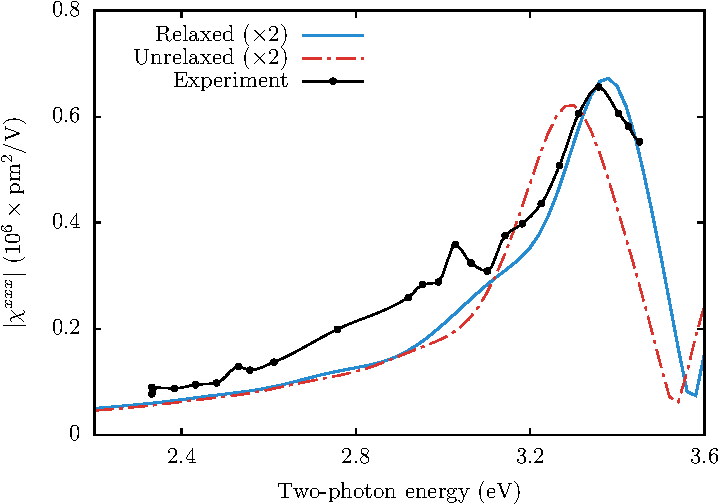
\includegraphics[width=0.8\textwidth]{../figures/04-results/fig-4_3_01}
\caption{Comparison of
$\chi_{\parallel\parallel\parallel}(-2\omega;\omega,\omega)$ calculated using
relaxed and unrelaxed atomic positions, with the experimental data presented in
Ref. \cite{hoferAPA96}. Theoretical curves are broadened with
$\sigma=0.075\,\text{eV}$. Experimental data was taken at 80 K.}
\label{fig:Xxxx}
\end{figure}

Therefore, the most accurate theoretical results are given by using relaxed atomic positions for the calculation of $\boldsymbol{\chi}(-2\omega;\omega,\omega)$. Although this process can be very time consuming for large numbers of atoms, we consider it a crucial step. From a numerical standpoint, this further demonstrates that SSHG is very sensitive to the surface atomic positions. In particular, our results show that a correct value of the Si-H bond length is not enough to obtain the most accurate SSHG spectra, and that a full relaxation of the structure is required. Additionally, the theory may coincide better with experiments that are conducted under very low temperature conditions.


%%%%%%%%%%%%%%%%%%%%%%%%%%%%%%%%%%%%%%%%%%%%%%%%%%%%%%%%%%%%%%%%%%%%%%%%%%%%%%%%
%%%%%%%%%%%%%%%%%%%%%%%%%%%%%%%%%%%%%%%%%%%%%%%%%%%%%%%%%%%%%%%%%%%%%%%%%%%%%%%%

\section{\texorpdfstring{Si(111)(1$\times$1):H}{Si(111)(1x1):H} -- Calculating the SSHG yield}


%%%%%%%%%%%%%%%%%%%%%%%%%%%%%%%%%%%%%%%%%%%%%%%%%%%%%%%%%%%%%%%%%%%%%%%%%%%%%%%%

\subsection{Calculated \texorpdfstring{$\mathcal{R}_{pS}$}{RpS} compared to experiment}\label{sec: RpS}

All calculations presented from this point on were done using the relaxed atomic positions described in previous sections. We now move on to the theoretical SSHG yield compared with experiment. We first compare the calculated $\mathcal{R}_{pS}$ spectra with room temperature experimental data from Ref. \cite{mejiaPRB02}. We adhere to the experimental setup by taking an angle of incidence $\theta=65^{\circ}$ and an azimuthal angle of $\phi=30^\circ$ with respect to the $x$-axis. This azimuthal angle maximizes $r_{pS}$, as shown in Eq. \eqref{eq:rpS}. In Fig. \ref{fig:RpS}, we see that all three models reproduce the lineshape of the experimental spectrum which includes the peaks corresponding to both the E$_{1}$ (3.4\,eV) and E$_{2}$ (4.3\,eV) critical points of bulk silicon, and a smaller feature at around 3.8\,eV. The calculated E$_{1}$ and E$_{2}$ peaks are redshifted by 0.1\,eV and 0.06\,eV, respectively, compared with the experimental peaks.


\begin{figure}
\centering
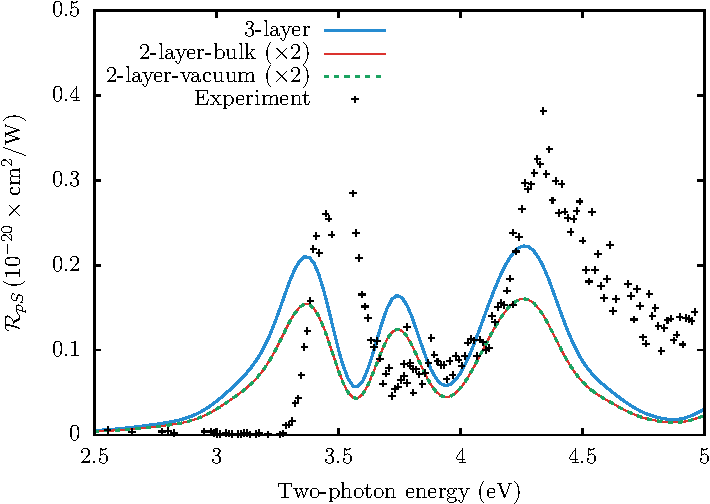
\includegraphics[width=0.8\textwidth]{../figures/04-results/fig-4_4_01}
\caption{Comparison between theoretical models (see Table
\ref{tab:models}) and experiment for $\mathcal{R}_{pS}$, for
$\theta=65^{\circ}$. We use a scissors value of $\hbar\Delta = 0.7\,\text{eV}$.
All theoretical curves are broadened with $\sigma=0.075\,\text{eV}$.
Experimental data taken from Ref. \cite{mejiaPRB02}, measured at room
temperature.}
\label{fig:RpS}
\end{figure}

The main issue to address here is the discrepancy between the intensity of the E$_{1}$ peak. In the theoretical curves, the peaks differ only slightly in overall intensity. Conversely, the experimental E$_{1}$ peak is significantly smaller than the E$_{2}$ peak. This may be due to the effects of oxidation on the surface. Ref. \cite{bergfeldPRL04} features similar data to those of Ref. \cite{mejiaPRB02} but focuses on the effects of surface oxidation. We can see that as time passes during the experiment, the surface becomes more oxidized, and the E$_{1}$ peak diminishes substantially, as shown by the experimental data taken 5 hours after initial H-termination. This may be enough time to slightly reduce the E$_{1}$ peak intensity, as can be observed here.

In Fig. \ref{fig:mitchellRpS}, we compare the theoretical $\mathcal{R}_{pS}$ with experimental data from Ref. \cite{mitchellSS01}; this data, however, only encompasses the E$_{1}$ peaks, and was obtained at room temperature. We consider an angle of incidence $\theta=45^\circ$ and an azimuthal angle $\phi=30^\circ$ to match these experimental conditions. As in the previous comparison, the E$_{1}$ peak is slightly redshifted compared to experiment. The intensity of the theoretical yield is smaller than the experimental yield for all three models. The measurements presented in Ref. \cite{mitchellSS01} were taken very shortly after the surface had been prepared, and the surface itself was prepared with a high degree of quality and measured at room temperature. Peak position compared to theory is slightly improved under these conditions. As before, the 3-layer model is closer in intensity to the experimental spectrum.

\begin{figure}
\centering
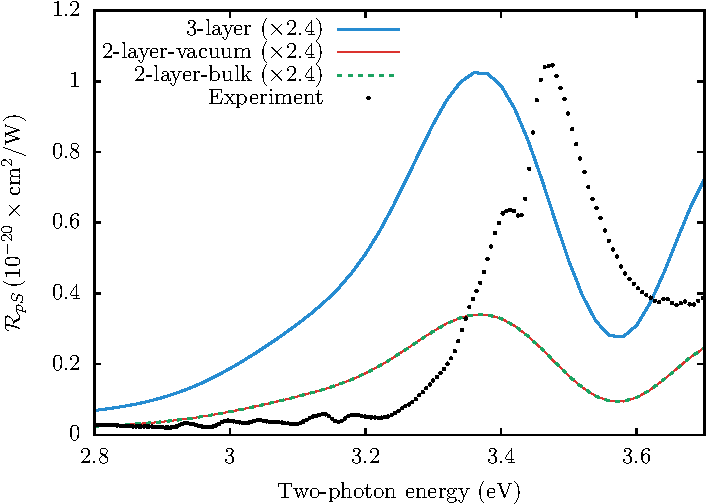
\includegraphics[width=0.8\textwidth]{../figures/04-results/fig-4_4_02}
\caption{Comparison between theoretical models (see Table
\ref{tab:models}) and experiment for $\mathcal{R}_{pS}$, for $\theta=45^\circ$.
We use a scissors value of $\hbar\Delta = 0.7\,\text{eV}$. All theoretical
curves are broadened with $\sigma=0.075\,\text{eV}$. Experimental data taken
from Ref. \cite{mitchellSS01}, measured at room temperature.}
\label{fig:mitchellRpS}
\end{figure}

We show in Fig.~\ref{fig:Xxxx} that our calculation for $\chi_{\parallel\parallel\parallel}(-2\omega;\omega,\omega)$ coincides with the measurement taken at a low temperature of 80 K. It is well known that temperature causes shifting in the peak position of SSHG spectra.\cite{dadapPRB97} As $\mathcal{R}_{pS}$ only depends on this component (see Eq.~\eqref{eq:rpS}), the position of the theoretical peak should be correct in Figs. \ref{fig:RpS} and \ref{fig:mitchellRpS}. We deduce that the difference in peak position stems from the higher  temperature at which the experiments were measured.

Both the 2-layer-vacuum and 2-layer-bulk models are identical and roughly 3 times smaller than the experiment. We can see from Eq. \eqref{eq:rpS} that $\mathcal{R}_{pS}$ only has $1\omega$ terms ($\varepsilon_{\ell}(\omega)$ and $k_{b}$). For both of these models, the fundamental fields are evaluated in the bulk, which means that the only change to Eq. \eqref{eq:rpS} is that $\varepsilon_{\ell}(\omega) \rightarrow \varepsilon_{b}(\omega)$. Additionally, $\Gamma^{\ell}_{pS}$ also remains identical between the two models and has no $2\omega$ terms in the denominator. Therefore, $r_{pS}$ is identical between these two models. Ultimately, the intensity of the 3-layer model is the closest to the experiment.

Per Eq. \eqref{eq:rpS}, the intensity of $\mathcal{R}_{pS}$ depends only on $\chi_{\parallel\parallel\parallel}$, which is not affected by local field effects.\cite{tancognedejean:tel-01235611} These effects are neglected in this calculation, but $\mathcal{R}_{pS}$ maintains an accurate lineshape and provides a good quantitative description of the experimental SSHG yield. We note that both the calculated and experimental spectra show two-photon resonances at the energies corresponding to the critical point transitions of bulk Si. We also see that the SSHG yield drops rapidly to zero below E$_{1}$, which is consistent with the absence of surface states due to the H saturation on the surface. This observation holds true for all three polarization cases studied here.

Lastly, in Fig. \ref{fig:improvements} we provide an overview of the different levels of approximation proposed in this article. All curves here were calculated using the 3-layer model. The long dashed line depicts the effect of excluding the contribution from the nonlocal part of the pseduopotentials. This is consistent with the results reported in Ref. \cite{andersonPRB15}, where the exclusion of this term increases the intensity of the components of $\boldsymbol{\chi}(-2\omega;\omega,\omega)$ by approximately 15\% to 20\%. We also notice that the E$_{1}$ peak is larger than the E$_{2}$ peak, contrasting with the experiment, where the E$_{1}$ peak is smaller than E$_{2}$. Lastly, the thin solid line depicts the full calculation with a scissors value of $\hbar\Delta = 0$. We notice that the spectrum is almost rigidly redshifted as this H-saturated surface has no electronic surface states.\cite{andersonPRB15} Thus, this demonstrates the importance of including the scissors correction to accurately reproduce the experimental spectrum. In summary, the inclusion of the contribution from the nonlocal part of the pseudopotentials and the scissors operator on top of the 3-layer model produces spectra with a lineshape and intensity that compare favorably with the experimental data.

\begin{figure}
\centering
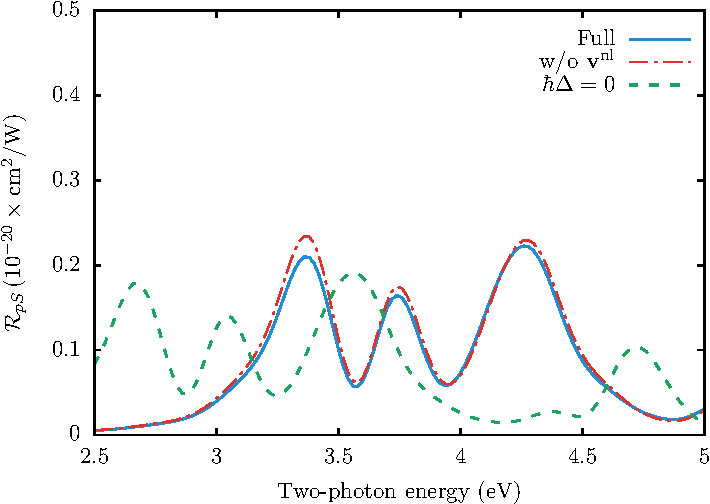
\includegraphics[width=0.8\textwidth]{../figures/04-results/fig-4_4_03}
\caption{Calculated results for $\mathcal{R}_{pS}$ for the
different levels of approximation proposed in this article. All curves were
calculated using the 3-layer model. We take $\theta=65^{\circ}$ for this plot.
See text for full details. All curves are broadened with
$\sigma=0.075\,\text{eV}$.
\label{fig:improvements}}
\end{figure}


%%%%%%%%%%%%%%%%%%%%%%%%%%%%%%%%%%%%%%%%%%%%%%%%%%%%%%%%%%%%%%%%%%%%%%%%%%%%%%%%

\subsection{Calculated \texorpdfstring{$\mathcal{R}_{sP}$}{RsP} compared to experiment}\label{sec:RsP}

Next, we analyze and compare the calculated $\mathcal{R}_{sP}$ spectra with experimental data from Ref. \cite{mejiaPRB02}. We again adhere to the experimental setup by taking an angle of incidence $\theta=65^{\circ}$ and an azimuthal angle $\phi=30^\circ$. From Fig. \ref{fig:RsP}, we can immediately appreciate that the overall intensity of $\mathcal{R}_{sP}$ is one order of magnitude lower than $\mathcal{R}_{pS}$. The experimental data is far noisier than in the other cases but we can still discern the E$_{1}$ and E$_{2}$ peaks. As with our previous comparisons, the 3-layer model is the closest match in both intensity and lineshape to the experimental spectrum. It produces a curve that is very close to the experimental intensity with good proportional heights for the calculated E$_{1}$ and E$_{2}$ peaks. In contrast, the 2-layer-vacuum model is 100 times more intense than experiment and produces an enlarged E$_{2}$ peak. The 2-layer-bulk model is ten times smaller with a very similar lineshape to the 3-layer model.

The differences between the 2-layer-vacuum and 2-layer-bulk models are not derived from Eq. \eqref{eq:rsP}, as the $\varepsilon_{b}(2\omega)$ does not change and the second term vanishes for this azimuthal angle of $\phi = 30$. However, $\Gamma^{\ell}_{sP}$ does cause a significant change in the intensity as there is an $\varepsilon_{\ell}(2\omega)$ term in the denominator. This will become $\varepsilon_{v}(2\omega) = 1$ for the 2-layer-vacuum model, and $\varepsilon_{b}(2\omega)$ in the bulk model. This accounts for the significant difference between the intensity of the two models, while the lineshape remains mostly consistent.

At higher energies, the theoretical curve is blueshifted as compared to the experiment. We consider that the likely explanation for this is the inclusion of the scissor operator, which does not adequately correct the transitions occurring at these higher energies. A full GW calculation would be well suited for this task, but is beyond the scope of this paper.

\begin{figure}
\centering
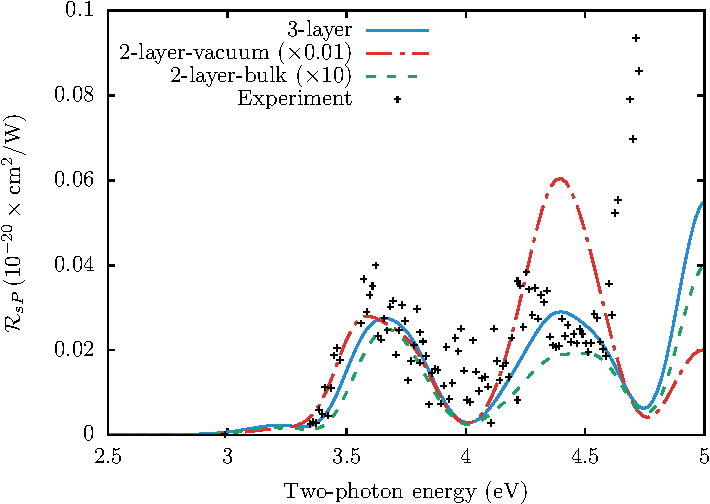
\includegraphics[width=0.8\textwidth]{../figures/04-results/fig-4_4_04}
\caption{Comparison between theoretical models (see Table
\ref{tab:models}) and experiment for $\mathcal{R}_{sP}$, for
$\theta=65^{\circ}$. We use a scissors value of $\hbar\Delta = 0.7\,\text{eV}$.
All theoretical curves are broadened with $\sigma=0.075\,\text{eV}$.
Experimental data taken from Ref. \cite{mejiaPRB02}, measured at room
temperature. \label{fig:RsP}}
\end{figure}


%%%%%%%%%%%%%%%%%%%%%%%%%%%%%%%%%%%%%%%%%%%%%%%%%%%%%%%%%%%%%%%%%%%%%%%%%%%%%%%%

\subsection{Calculated \texorpdfstring{$\mathcal{R}_{pP}$}{RpP} compared to
experiment}\label{sec:RpP}

We present $\mathcal{R}_{pP}$ compared to experimental data from Ref. \cite{mejiaPRB02} in Fig. \ref{fig:RpP}. We note that peak position for the 3-layer model is similar to experiment with the overall intensity being only two times larger. The E$_{2}$ peak is blueshifted by around 0.3\,eV, and the yield does not go to zero after 4.75\,eV. The 2-layer-vacuum model produces a spectrum with peak positions that are close to the experiment, but are 40 times more intense. The calculated E$_{2}$ peak is similar, but the E$_{1}$ peak lacks the sharpness present in the experiment. The 2-layer-bulk model is very close to the lineshape of the 3-layer model, but with eight times less intensity. From Eq. \eqref{eq:rpP}, we see that $\mathcal{R}_{pP}$ has several $2\omega$ terms that will change between models; this will have a deep effect on the lineshape. Additonally, $\Gamma^{\ell}_{pP}$ also has $\varepsilon_{\ell}(2\omega)$ in the denominator, and so we have a significant difference in both lineshape and intensity between the 2-layer-vacuum and the other two models. Again, as in the previous sections for $\mathcal{R}_{pS}$ and $\mathcal{R}_{sP}$, the 3-layer model is the closest in intensity to the experiment. Additionally, Ref. \cite{dadapPRB97} shows that low temperature measurements of $\mathcal{R}_{pP}$ will blueshift the spectrum away from room temperature measurements such as those shown in Figs. \ref{fig:RpP} and \ref{fig:mitchellRpP}, and towards our theoretical results.

Reviewing Eq. \eqref{eq:rpP}, we see that $\mathcal{R}_{pP}$ is by far the most involved calculation, since it includes all four nonzero components. In particular, $\chi_{\perp\perp\perp}$ and $\chi_{\parallel\parallel\perp}$ include out-of-plane incoming fields. These are affected by local field effects\cite{tancognedejean:tel-01235611} that reveal the inhomogeneities in the material, which are by far more prevalent perpendicular to the surface than in the surface plane. This can be evidenced for Si, as Reflectance Anisotropy Spectroscopy (RAS) measurements are well described by \emph{ab initio} calculations neglecting local field effects.\cite{palummoPRB99, gaalPRB09} It is therefore expected that the out-of-plane components will be more sensitive to the inclusion of local fields. These will not change the transition energies, only their relative weights of the resonant peaks,\cite{tancognedejean:tel-01235611} but including these effects is challenging to compute,\cite{nicolasPRB15} and beyond the scope of this paper. We speculate that $\mathcal{R}_{pP}$ requires the proper inclusion of these effects in order to accurately describe the experimental peaks.

\begin{figure}
\centering 
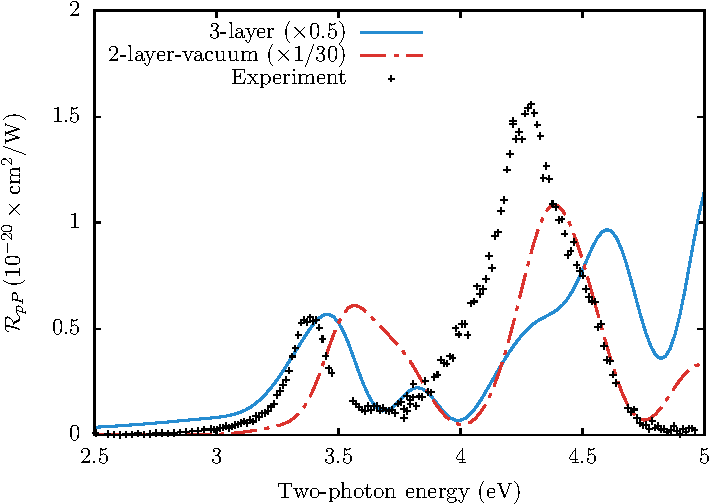
\includegraphics[width=0.8\textwidth]{../figures/04-results/fig-4_4_05}
\caption{Comparison between theoretical models (see Table
\ref{tab:models}) and experiment for $\mathcal{R}_{pP}$, for
$\theta=65^{\circ}$. We use a scissors value of $\hbar\Delta = 0.7\,\text{eV}$.
All theoretical curves are broadened with $\sigma=0.075\,\text{eV}$.
Experimental data taken from Ref. \cite{mejiaPRB02}, measured at room
temperature. \label{fig:RpP}}
\end{figure}

\begin{figure}
\centering 
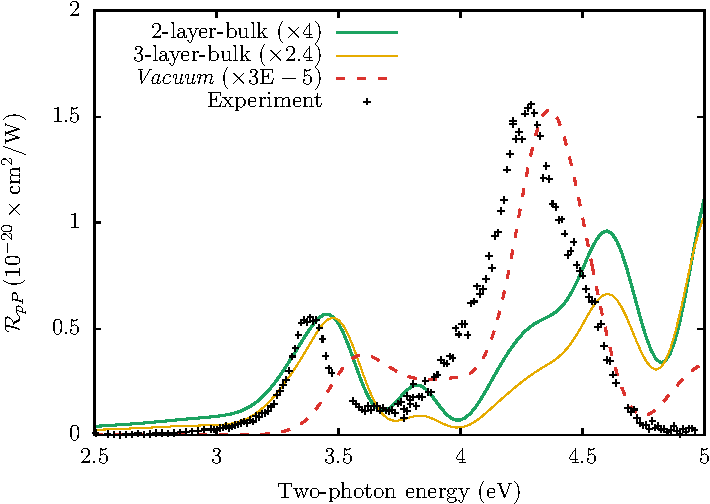
\includegraphics[width=0.8\textwidth]{../figures/04-results/fig-4_4_06}
\caption{Other models. \label{fig:RpP}}
\end{figure}

In Fig. \ref{fig:mitchellRpP} we compare to Ref. \cite{mitchellSS01}. The 3-layer model is, as before, close to the experiment in both peak position and intensity. Intensity is almost the same the experimental value. This provides a more compelling argument against the 2-layer-vacuum model than Fig. \ref{fig:RpP}. The 2-layer-vacuum model is 20 times more intense and blueshifted by around 0.1\,eV. As mentioned before, this surface is of very high quality with measurements taken shortly after surface preparation. As before, the 2-layer-bulk model is intermediate between the other two models in both intensity and lineshape. Under these conditions, the 3-layer model very accurately reproduces the E$_{1}$ peak over the 2-layer-vacuum and 2-layer-bulk models.

\begin{figure}
\centering
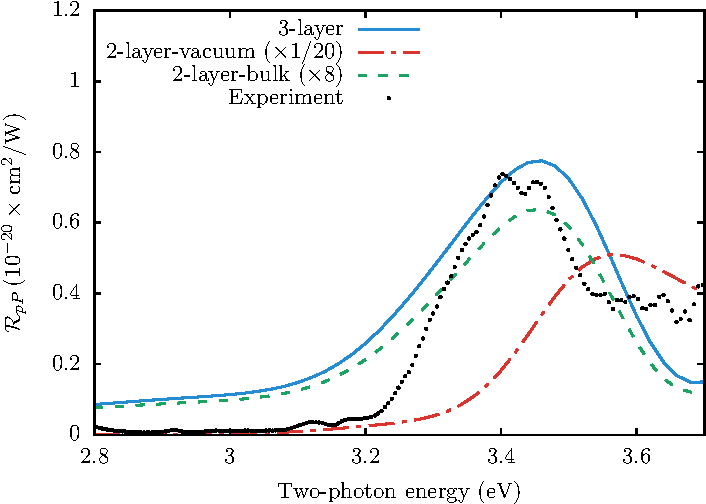
\includegraphics[width=0.8\textwidth]{../figures/04-results/fig-4_4_07}
\caption{Comparison between theoretical models (see Table
\ref{tab:models}) and experiment for $\mathcal{R}_{pP}$, for
$\theta=45^{\circ}$. We use a scissors value of $\hbar\Delta = 0.7\,\text{eV}$.
All theoretical curves are broadened with $\sigma=0.075\,\text{eV}$.
Experimental data taken from Ref. \cite{mitchellSS01}, measured at room
temperature.}
\label{fig:mitchellRpP}
\end{figure}

Lastly, for linear optics and SHG, $GW$ transition energies are needed. Doing a Bethe-Salpeter calculation for SSHG will improve the position and the amplitude of the peaks, but is far beyond current capabilities.\cite{puff} We did not adjust the value of the scissors shift, as we want to keep our calculation at the {\em ab initio} level. We remark again that the choice of $\hbar\Delta=0.7$ eV for the scissors shift comes from a $GW$ calculation.\cite{liPRB10} As explained in Fig. \ref{fig:improvements}, the lack of surface states causes an almost rigid shift of the spectra by applying the scissors correction. We have checked that it is not possible to have a single scissors value that can reproduce the energy positions of both the E$_{1}$ and the E$_{2}$ peaks. Of course, the experimental temperature at which the spectra is measured should be taken into account in a more complete formulation. However, we have restricted our calculation to $T=0$ K.

\begin{figure}
    \begin{minipage}[b]{0.5\textwidth}
        \centering
        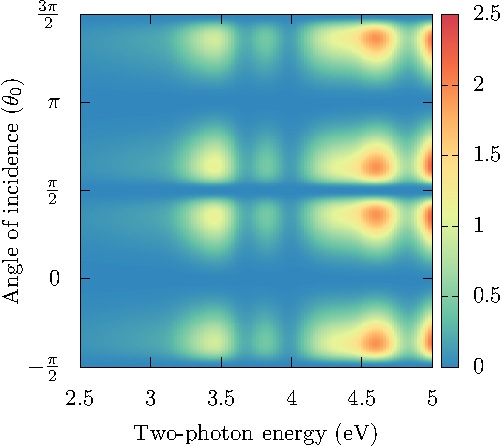
\includegraphics[height=6cm]{../figures/04-results/fig-4_4_08}
        \subcaption{$\mathcal{R}_{pP}$}\label{fig:1x1rpp3d}
    \end{minipage}
    ~
    \begin{minipage}[b]{0.5\textwidth}
        \centering
        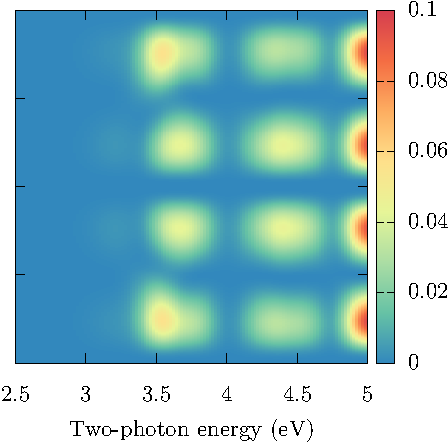
\includegraphics[height=5.945cm]{../figures/04-results/fig-4_4_09}
        \subcaption{$\mathcal{R}_{sP}$}\label{fig:1x1rsp3d}
    \end{minipage}
    \caption{$\mathcal{R}$ for outgoing $P$ polarized fields, versus the angle
    of incidence ($\theta_{0}$) for the Si(111)(1$\times$1):H surface. Both
    figures consider an azimuthal angle of $\phi = 45^{\circ}$. All curves are
    broadened with $\sigma = 0.075$ eV.}
    \label{fig:1x1rP3d}
\end{figure}

\begin{figure}
    \begin{minipage}[b]{0.5\textwidth}
        \centering
        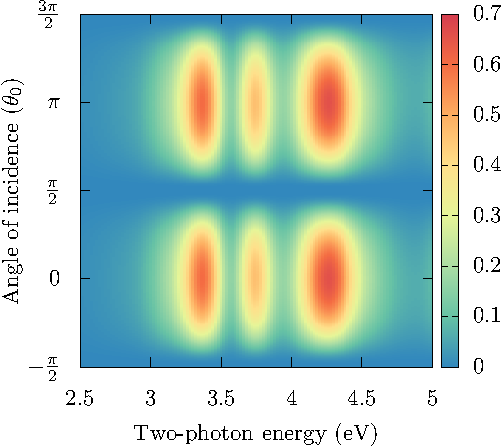
\includegraphics[height=6cm]{../figures/04-results/fig-4_4_10}
        \subcaption{$\mathcal{R}_{pS}$}\label{fig:1x1rps3d}
    \end{minipage}
    ~
    \begin{minipage}[b]{0.5\textwidth}
        \centering
        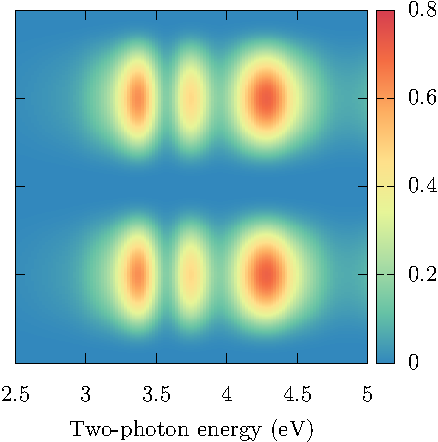
\includegraphics[height=5.945cm]{../figures/04-results/fig-4_4_11}
        \subcaption{$\mathcal{R}_{sS}$}\label{fig:1x1rss3d}
    \end{minipage}
    \caption{$\mathcal{R}$ for outgoing $S$ polarized fields, versus the angle
    of incidence ($\theta_{0}$) for the Si(111)(1$\times$1):H surface. Both
    figures consider an azimuthal angle of $\phi = 45^{\circ}$. All curves are
    broadened with $\sigma = 0.075$ eV.}
    \label{fig:1x1rS3d}
\end{figure}


%%%%%%%%%%%%%%%%%%%%%%%%%%%%%%%%%%%%%%%%%%%%%%%%%%%%%%%%%%%%%%%%%%%%%%%%%%%%%%%%

\subsection{Calculating \texorpdfstring{$\mathcal{R}_{\mathrm{iF}}$}{Rif}
including the effects of multiple reflections}

We consider a Si(111)(1$\times$1):H surface as a test case for the three layer model and to study the effects that multiple reflections have on the SSHG radiation. This surface is well characterized experimentally,\cite{mitchellSS01, mejiaPRB02, bergfeldPRL04} and there has been success in reproducing these experimental results using the three layer model without multiple reflections.\cite{andersonPRB16} The details of the \emph{ab initio} calculation of $\chi_{ijk}$ are not needed for the following discussion, and are left for the reader in Ref. \cite{andersonPRB16}. However, we mention that we apply a scissors shift of 0.7 eV to the theoretical spectra. In a first approximation, this includes the effects of the electronic many-body interactions within the independent particle approach for the \emph{ab initio} calculation. This 0.7 eV value allows the SH resonant peaks to acquire their corresponding energy positions, and is calculated with what is known as a $G_{0}W_{0}$ calculation.\cite{andersonPRB16} As mentioned in Sec. \ref{sec:intro}, we are interested in finding the thickness of the layer $\ell$ where $\chi_{ijk} \ne 0$. For this surface, we found well-converged results for a thickness of $\sim 5$ nm, that is equivalent to 24 atomic sheets of Si along the (111) direction. As this represents only the upper half of the slab, we find it reasonable to choose the thickness of the layer $\ell$ to be between $d\sim 5-10$ nm. This corresponds to a half-slab comprised of 24 to 48 atomic layers to get well-converged values of $\chi_{ijk}$.

In Fig. \ref{fig:d2values}, we compare the theoretical results for the SSHG yield with the experimental results from Ref. \cite{mejiaPRB02}. We mention that the experimental results where produced with an angle of incidence of $\theta=65^\circ$, and an azimuthal angle of $\phi=30^\circ$, which eliminates the contribution from $\chi_{xxx}$ from Eq. \eqref{rpp111}. First, we note that the experimental spectrum shows two very well defined resonances which come from electronic transitions from the valence to the conduction bands around the well known $E_{1}\sim 3.4$ eV and $E_{2}\sim 4.3$ eV critical points of Si.\cite{yubook} As can be seen, the theoretical results reproduce the features of the spectrum, although we see that the $E_{2}$ peak is blueshifted by around 0.3\,eV. Here we focus on the SSHG yield itself rather than on the physics that lead to such a blueshifted theoretical spectrum. The interested reader can refer to Ref. \cite{andersonPRB16} for those details.

All curves in this figure that include multiple reflections consider $d = 10$ nm. We compare the theoretical SSHG yield for $d_{2} = 0$ nm and $d_{2} = 10$ nm, with the SSHG yield that neglects multiple reflections. When $d_{2} = 0$ nm, we have placed the polarization sheet at the bottom of the layer region. This minimizes the effect of the multiple reflections, and thus the curve is very similar to the three layer model that neglects multiple reflections entirely. When $d_{2} = 10$ nm, the polarization sheet is placed at the top of the layer region. This maximizes the effect of the multiple reflections and therefore leads to the largest yield. We also notice that the average value obtained by using $\bar{R}^{M}_{i}$ (Eq. \eqref{mcave}) is intermediate between $d_{2} = 0$ and $d_{2} = 10$ nm, as expected. This is very similar to selecting $d_{2} = d/2$, which can be interpreted as placing the nonlinear polarization sheet $\mathbf{P}(\mathbf{r},t)$ at the middle of layer $\ell$. It is important to remark that these enhancements are larger for $E_{2}$ than for $E_{1}$. This can be understood from the fact that the corresponding $\lambda_{0}$ for $E_{1}$ is larger than that of $E_{2}$. From Eqs. \eqref{delta0}, \eqref{delta}, and \eqref{mphi}, we see that the phase shifts are larger for $E_{2}$ than for $E_{1}$, producing a larger enhancement of the SSHG yield at $E_{2}$ from the multiple reflections. As the phase shifts grow with $d$, so does the enhancement caused by the multiple reflections. We have verified that the effects of the multiple reflections from the linear field are significantly smaller than those of the SH field. This is clear since the phase shift of Eq. \eqref{mphi} is not only a factor of 2 smaller than that of Eqs. \eqref{delta0} and \eqref{delta}, but also $w_\ell < W_\ell$.

From this figure, it becomes evident that the inclusion of multiple reflections is crucial to obtain a better agreement between the theoretical SSHG yield and the experimental spectrum. This is particularly true for larger energies, such as $E_{2}$, as $\lambda_{0}$ becomes smaller and the multiple reflection effects become more noticeable. The selected value for $d << \lambda_{0}$, that comes naturally from the \emph{ab initio} calculation of $\chi_{ijk}$ is thus very reasonable in order to model a thin surface layer below the vacuum region where the nonlinear SH conversion takes place.

\begin{figure}
\centering
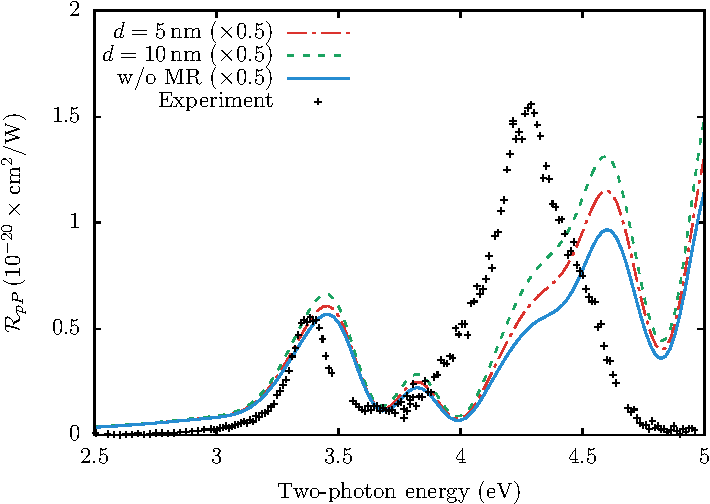
\includegraphics[width=0.8\textwidth]{../figures/04-results/fig-4_4_12}
\caption{Comparison between theoretical models (see Table
\ref{tab:models}) and experiment for $\mathcal{R}_{pP}$, for
$\theta=45^{\circ}$. We use a scissors value of $\hbar\Delta = 0.7\,\text{eV}$.
All theoretical curves are broadened with $\sigma=0.075\,\text{eV}$.
Experimental data taken from Ref. \cite{mitchellSS01}, measured at room
temperature.}
\label{fig:mr1}
\end{figure}

\begin{figure}
\centering
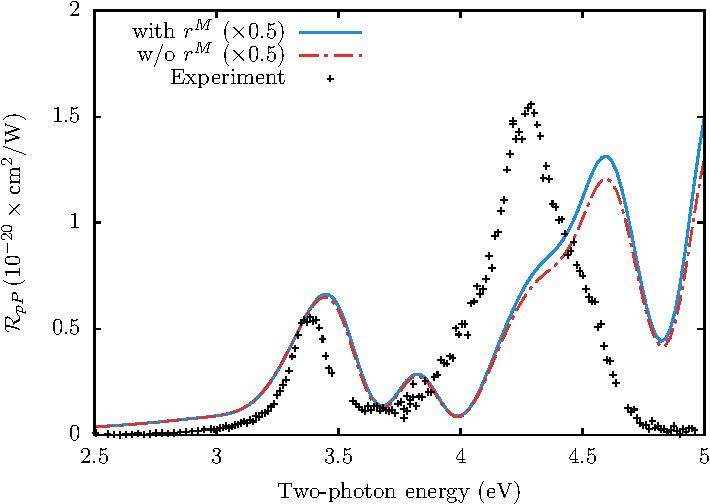
\includegraphics[width=0.8\textwidth]{../figures/04-results/fig-4_4_13}
\caption{Comparison between theoretical models (see Table
\ref{tab:models}) and experiment for $\mathcal{R}_{pP}$, for
$\theta=45^{\circ}$. We use a scissors value of $\hbar\Delta = 0.7\,\text{eV}$.
All theoretical curves are broadened with $\sigma=0.075\,\text{eV}$.
Experimental data taken from Ref. \cite{mitchellSS01}, measured at room
temperature.}
\label{fig:mr2}
\end{figure}

\begin{figure}
\centering
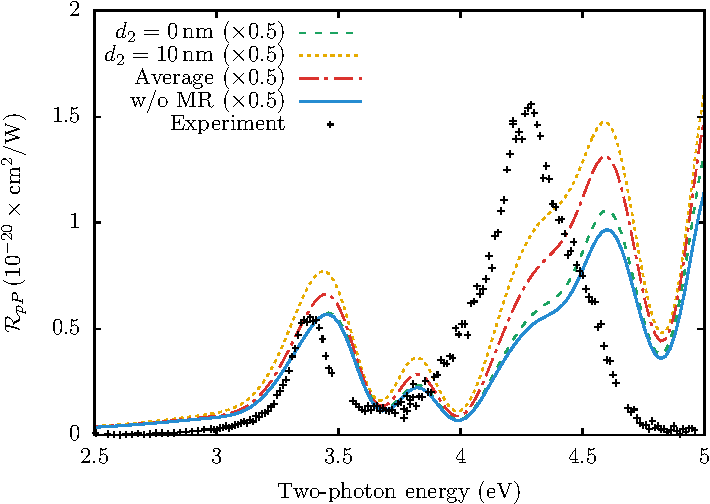
\includegraphics[width=0.8\textwidth]{../figures/04-results/fig-4_4_14}
\caption{Comparison between theoretical models (see Table
\ref{tab:models}) and experiment for $\mathcal{R}_{pP}$, for
$\theta=45^{\circ}$. We use a scissors value of $\hbar\Delta = 0.7\,\text{eV}$.
All theoretical curves are broadened with $\sigma=0.075\,\text{eV}$.
Experimental data taken from Ref. \cite{mitchellSS01}, measured at room
temperature.}
\label{fig:mr3}
\end{figure}


\bibliographystyle{unsrt}
\bibliography{/Users/sma/Dropbox/docs/academics/master}

\end{document}
